\documentclass[a4paper,14pt]{extreport}
	\usepackage[left=1.5cm,right=1.5cm,
	    top=1.5cm,bottom=2cm,bindingoffset=0cm]{geometry}
	\usepackage{scrextend}
	\usepackage[T1,T2A]{fontenc}
	\usepackage[utf8]{inputenc}
	\usepackage[english,russian,ukrainian]{babel}
	\usepackage{tabularx}
	\linespread{1.5}
	\usepackage{amssymb}
	\usepackage{fp}
	\usepackage{color}
	\usepackage{amsmath}
	\usepackage{mathrsfs}
	\usepackage{listings}
	\usepackage{graphicx}
	\graphicspath{ {./images/} }
	\usepackage{lipsum}
	\usepackage{xcolor}
	\usepackage{multirow}
	%\usepackage[table,xcdraw]{xcolor}
	\usepackage{hyperref}
	\usepackage{tcolorbox}
	\usepackage{tikz}
	\usepackage[framemethod=TikZ]{mdframed}
	\usepackage{wrapfig,boxedminipage,lipsum}
	\mdfdefinestyle{MyFrame}{%
	linecolor=blue,outerlinewidth=2pt,roundcorner=20pt,innertopmargin=\baselineskip,innerbottommargin=\baselineskip,innerrightmargin=20pt,innerleftmargin=20pt,backgroundcolor=gray!50!white}
	 \usepackage{csvsimple}
	 \usepackage{supertabular}
	\usepackage{pdflscape}
	\usepackage{fancyvrb}
	%\usepackage{comment}
	\definecolor{ggreen}{rgb}{0.4,1,0}
	\definecolor{rred}{rgb}{1,0.1,0.1}
	\definecolor{aquamarine}{rgb}{0.5, 1.0, 0.83}
	\definecolor{amber}{rgb}{1.0, 0.75, 0.0}
	\definecolor{babyblue}{rgb}{0.54, 0.81, 0.94}
	\definecolor{buff}{rgb}{0.94, 0.86, 0.51}
	\definecolor{internationalorange}{rgb}{1.0, 0.31, 0.0}
	\definecolor{lightmauve}{rgb}{0.86, 0.82, 1.0}
	\definecolor{mediumaquamarine}{rgb}{0.4, 0.8, 0.67}
	\usepackage{array,tabularx}
	\usepackage{colortbl}
	
	\usepackage{varwidth}
	\tcbuselibrary{skins}
	\usepackage{fancybox}

	\usetikzlibrary{calc}
	\makeatletter
	\newlength{\mylength}
	\xdef\CircleFactor{1.1}
	\setlength\mylength{\dimexpr\f@size pt}
	\newsavebox{\mybox}
	\newcommand*\circled[2][draw=blue]{\savebox\mybox{\vbox{\vphantom{WL1/}#1}}\setlength\mylength{\dimexpr\CircleFactor\dimexpr\ht\mybox+\dp\mybox\relax\relax}\tikzset{mystyle/.style={circle,#1,minimum height={\mylength}}}
	\tikz[baseline=(char.base)]
	\node[mystyle] (char) {#2};}
	\makeatother
	\usepackage{pgfplots}
    \pgfplotsset{compat=1.9}


	\usepackage{float}
	\usepackage{wrapfig}
	\usepackage{framed}
	%for nice Code{
	\lstdefinestyle{customc}{
	  belowcaptionskip=1\baselineskip,
	  breaklines=true,
	  frame=L,
	  xleftmargin=\parindent,
	  language=C,
	  showstringspaces=false,
	  basicstyle=\small\ttfamily,
	  keywordstyle=\bfseries\color{green!40!black},
	  commentstyle=\itshape\color{purple!40!black},
	  identifierstyle=\color{blue},
	  stringstyle=\color{orange},
	}
	\lstset{escapechar=@,style=customc}
	\usepackage{enumitem}
%}


\begin{document}
\newtcbox{\xmybox}[1][red]{on line, arc=7pt,colback=#1!10!white,colframe=#1!50!black, before upper={\rule[-3pt]{0pt}{10pt}},boxrule=1pt, boxsep=0pt,left=6pt,right=6pt,top=2pt,bottom=2pt}
\pagecolor{white}
\begin{titlepage}
	\begin{center}
	\large
	Національний технічний університет України \\ "Київський політехнічний інститут імені Ігоря Сікорського"


	Факультет Електроніки

	Кафедра мікроелектроніки
	\vfill

	\textsc{ЗВІТ}\\

	{\Large Про виконання РГР\\
	з дисципліни: «Вакуумна та плазмова електроніка»\\[1cm]

	


	}
	\bigskip
	\end{center}
	\vfill

	\newlength{\ML}
	\settowidth{\ML}{«\underline{\hspace{0.4cm}}» \underline{\hspace{2cm}}}
	\hfill
	\begin{minipage}{1\textwidth}
	Виконавець:\\
	Студент 3-го курсу \hspace{4cm} $\underset{\text{(підпис)}}{\underline{\hspace{0.2\textwidth}}}$  \hspace{1cm}В.\,О.~Тололо\\


	Перевірив: \hspace{5.9cm} $\underset{\text{(підпис)}}{\underline{\hspace{0.2\textwidth}}}$  \hspace{1cm}О.\,М.~Бевза\\

	\end{minipage}

	\vfill

	\begin{center}
	2021
	\end{center}
\end{titlepage}

\begin{center}\textbf{Завдання}\end{center}\par
	\begin{enumerate}
		\item 	Дивимось на графіки побудовані для п.3 лабораторної роботи.
		\begin{enumerate}[label=1.\arabic*]
			\item Визначити частоту червоної границі фотоефекту.
			\item Необхідно визначити напругу запирання для кожного елементу при інтенсивності 50 \% та 100\%.  Пояснити, чому напруги запирання відрізняються при різній інтенсивності.
			\item  Побудувати графіки залежностей напруги запирання від частоти ( у вас вказані довжини хвиль, отже їх треба перерахувати в частоту) для випадку інтенсивності 50\% та 100\%.  Для кожного матеріалу (у кожного свої три матеріала).
			\item Визначити з цих нових побудованих графіків роботу виходу в точці (будь-якій, назвіть її А) за вашим власним вибором, яка розташована десь посередині отриманого графіку. Для всіх трьох матеріалів. Для обох значень інтенсивності (50\% та 100\%). Порівняйте отримані значення роботи виходу при двох різних інтенсивностей для кожного матеріалу та зробити висновки.
			\item  Розрахувати кінетичну швидкість електронів для точки А для всіх трьох матеріалів.
			\item  Порівняти отримане із розрахунку значення роботи виходу з відомими значеннями роботи виходу (довідкові дані, вказати джерело) та розрахувати абсолютну та відносну помилки. Зробити для трьох ваших матеріалів матеріалів.
			\item  Отримані результати звести до таблиці, де повинен бути вказаний кожен з трьох матеріалів та розраховані для нього значення: частота червоної границі фотоефекту, напруга запирання (для двох інтенсивностей), робота виходу в точці А (дві інтенсивності), кінетична швидкість електронів в точці А (для двох інтенсивностей 50\% та 100\%).
			\item Зробіть перевірку правильності виконання розрахунків за формулою Ейнштейна для фотоефекту.
		\end{enumerate}

		\item Беремо  графіки зроблені до пункту 4, де було побудовано залежності струму від інтенсивності. Ви вибирали самі три довжини хвилі. У кожного вибрано свій один матеріал. Робимо:
		\begin{enumerate}[label=2.\arabic*]
			\item Побудуйте ваш графік в інших координатах, де вісь х- довжина хвилі, вісь у-струм. Беремо значення струму для Інтенсивності 50\%.
			\item Побудуйте самі (ваші припущення) на вашому новому графіку іншим кольором як буде виглядати ця залежність, якщо інтенсивність буде складати, а далі за списком вибираємо свій варіант.
		\end{enumerate}
		\item Пояснити чому струм змінився саме так. Дивимось на графіки побудовані для пункта 5. Де залежності енергії від частоти. Треба:
		\begin{enumerate}[label=3.\arabic*]
			\item Визначити яка саме енергія стоїть у вас по осі ігрек. Це повна енергія фотону чи робота виходу чи кінетична енергія електрона чи щось інше? Відповідь аргументовано пояснити.
		\end{enumerate}
\end{enumerate}
\newpage
%\begin{center}\textbf{\fbox{Виконання роботи}}\end{center}\par
	
%-----------------------------------------1.1
\begin{center}
\textbf{Завдання 1}
\end{center}


Частотa червоної межі фотоефекту для Na $\approx  0.5 \cdot 10^{15}$ Гц \\
Частотa червоної межі фотоефекту для Zn $\approx  1.1 \cdot 10^{15}$ Гц \\
Частотa червоної межі фотоефекту для Cа $\approx  0.75 \cdot  10^{15}$ Гц\\ 
	
%-----------------------------------------1.2-1.3

	За формулою $v = \dfrac{c}{\lambda}$ можна знайти частоту наступним чином:
	
	
	\begin{table}[h]
		\begin{center}
			\begin{tabular}{|c|c|}
			\hline
			$\lambda$, нм & $f \cdot 10^{15}$,  Гц \\ \hline
			200               & 1,5                   \\ \hline
			400               & 0,7                  \\ \hline
			440               & 0,6                \\ \hline
			470               & 0,6                  \\ \hline
			\end{tabular}
		\end{center}
	\end{table}
	
			Тепер побудую графіки залежностей напруги запирання від частоти для випадку інтенсивності 50\% та 100\%, для кожного матеріалу	

	
			
		
	\begin{center}

	\begin{minipage}{0.4\textwidth}
			\begin{center}
				\begin{tabular}{|c|c|c|}
					\hline
					\multicolumn{3}{|c|}{Na} \\ \hline
					 & \multicolumn{2}{c|}{$U_{\text{з}}$, B} \\ \cline{2-3} 
					\multirow{-2}{*}{$f\cdot 10^{15}$, Гц} & 50\% & 100\% \\ \hline
					 & 50\% & 100\%    \\ \hline
					0.6 &  0   &  0    \\ \hline
					0.6 & -0.4 & -0.4  \\ \hline
					0.7 & -0.8 & -0.6  \\ \hline
					1.5 & -4   & -4.1    \\ \hline
				\end{tabular}
			\end{center}
		\end{minipage}
		\hfill
		\begin{minipage}{0.4\textwidth}
		\begin{tikzpicture}%Na
			\begin{axis}[table/col sep = semicolon,
			title={Na},
			xlabel = {$f\cdot 10^{15},\text{ Гц}$},
			ylabel = {$U_{\text{з}}, B$},
			height = 0.25\paperheight, 
			width =  0.25\paperwidth,
			%legend pos = north west,
			ymajorgrids=true,
			xmajorgrids=true,
			grid style=dashed,
			legend style={nodes={scale=0.7, transform shape}}]
			\legend{ 
			\text{50\%}, \text{100\%}};
			\addplot [green,mark=+] table [ x={b},y={c}]{1.2-1.3.csv};
			\addplot  [orange,mark=+] table [x={b},y={d}]{1.2-1.3.csv};
			\end{axis}
		\end{tikzpicture}
	\end{minipage}
	
	\begin{minipage}{0.4\textwidth}
			  \begin{center}
			\begin{tabular}{|c|c|c|}
					\hline
					\multicolumn{3}{|c|}{ Zn} \\ \hline
					\multirow{2}{*}{$f\cdot 10^{15}$, Гц} & \multicolumn{2}{c|}{$U_{\text{з}}$, B} \\ \cline{2-3} 
					 & 50\% & 100\% \\ \hline
					0.6 &0 &0 \\ \hline
					0.6 &0 &0 \\ \hline
					0.7 &0 &0\\ \hline
					1.5 & -1.92 & -2.5 \\ \hline
				\end{tabular}
			\end{center}
			\end{minipage}
			\hfill
			\begin{minipage}{0.4\textwidth}
			  \begin{tikzpicture}
			\begin{axis}[table/col sep = semicolon,
			title={Ca},
			xlabel = {$f\cdot 10^{15},\text{ Гц}$},
			ylabel = {$U_{\text{з}}, B$},
			height =  0.25\paperheight, 
			width =  0.25\paperwidth,
			ymajorgrids=true,
			xmajorgrids=true,
			grid style=dashed,
			legend style={nodes={scale=0.7, transform shape}}]
			\legend{ 
			\text{50\%}, \text{100\%}};
			\addplot [green,mark=+]table [grid style = both, x={g},y={h}]{1.2-1.3.csv};
			\addplot [red,mark=+]table [grid style = both, x={g},y={i}]{1.2-1.3.csv};
			\end{axis}
		\end{tikzpicture}
	\end{minipage}

	\begin{minipage}{0.4\textwidth}
		  		\begin{center}
			\begin{tabular}{|c|c|c|}
					\hline
					\multicolumn{3}{|c|}{ Cu} \\ \hline
					\multirow{2}{*}{$f\cdot 10^{15}$, Гц} & \multicolumn{2}{c|}{$U_{\text{з}}$, B} \\ \cline{2-3} 
					 & 50\% & 100\%    \\ \hline
					0.6 &  0   &  0    \\ \hline
					0.6 & 0 & 0  \\ \hline
					0.7 & 0 & 0  \\ \hline
					1.5 & -6.2   & -6.9    \\ \hline
				\end{tabular}
			\end{center}
			
		\end{minipage}
		\hfill
		\begin{minipage}{0.4\textwidth}
		  	\begin{tikzpicture}%Cu
			\begin{axis}[table/col sep = semicolon,
				title={Cu},
				xlabel = {$f\cdot 10^{15},\text{ Гц}$},
				ylabel = {$U_{\text{з}}, B$},
				height = 0.25\paperheight, 
				width = 0.25\paperwidth,
				ymajorgrids=true,
				xmajorgrids=true,
	    		grid style=dashed,
	    		legend style={nodes={scale=0.7, transform shape}}]
				\legend{ 
				\text{50\%}, \text{100\%}};
				\addplot[black,mark=+] table [grid style = both, x={l},y={m}]{1.2-1.3.csv};
				\addplot[red,mark=+] table [grid style = both, x={l},y={n}]{1.2-1.3.csv};
			\end{axis}
		\end{tikzpicture}%Cu
	\end{minipage}
		
	\end{center}


%\\\\\\\\\\\\\\\\\\\\\\\\\\\\\\\\\\\\\\\\\\\\\\\\\\\\\\\\\%\\\\\\\\\\\\\\\\\\\\\\\\\\\\\\\\\\\\\\\\\\\\\\\\\\\\\\\\\%\\\\\\\\\\\\\\\\\\\\\\\\\\\\\\\\\\\\\\\\\\\\\\\\\\\\\\\\\%\\\\\\\\\\\\\\\\\\\\\\\\\\\\\\\\\\\\\\\\\\\\\\\\\\\\\\\\\%\\\\\\\\\\\\\\\\\\\\\\\\\\\\\\\\\\\\\\\\\\\\\\\\\\\\\\\\\%\\\\\\\\\\\\\\\\\\\\\\\\\\\\\\\\\\\\\\\\\\\\\\\\\\\\\\\\\%\\\\\\\\\\\\\\\\\\\\\\\\\\\\\\\\\\\\\\\\\\\\\\\\\\\\\\\\\%\\\\\\\\\\\\\\\\\\\\\\\\\\\\\\\\\\\\\\\\\\\\\\\\\\\\\\\\\%\\\\\\\\\\\\\\\\\\\\\\\\\\\\\\\\\\\\\\\\\\\\\\\\\\\\\\\\\%\\\\\\\\\\\\\\\\\\\\\\\\\\\\\\\\\\\\\\\\\\\\\\\\\\\\\\\\\%\\\\\\\\\\\\\\\\\\\\\\\\\\\\\\\\\\\\\\\\\\\\\\\\\\\\\\\\\%\\\\\\\\\\\\\\\\\\\\\\\\\\\\\\\\\\\\\\\\\\\\\\\\\\\\\\\\\%\\\\\\\\\\\\\\\\\\\\\\\\\\\\\\\\\\\\\\\\\\\\\\\\\\\\\\\\\
%-----------------------------------------1.4
	
		Тепер з побудованих графіків треба визначити роботу виходу в точці А, яка розташована десь посередині отриманих графіків, для всіх трьох матеріалів. $A = h\cdot f$
	

	\FPeval\na{round( 4.14*1  :3)}
	\FPeval\naa{round( 4.14*1 :3)}

	\FPeval\zn{round( 4.14*1.  :3)}
	\FPeval\znn{round( 4.14*1.1  :3)}

	\FPeval\cu{round( 4.14*1.1  :3)}
	\FPeval\cuu{round( 4.14*1.2  :3)}


	\begin{align*}
		A_{Na-50\%} &= \na \text{ eB}\\
		A_{Na-100\%} &= \naa \text{ eB}\\
		A_{Zn-50\%} &= \zn \text{ eB}\\
		A_{Zn-100\%} &= \znn \text{ eB}\\
		A_{Cu-50\%} &= \cu \text{ eB}\\
		A_{Cu-100\%} &= \cuu \text{ eB}\\
	\end{align*}
%-----------------------------------------1.5
 

	Pахуємо кінетичну швидкість електронів для точки А для всіх трьох матеріалів:
	\begin{equation}
		v = \sqrt{ \dfrac{2\cdot e\cdot U_{\text{з}}}{m} }
	\end{equation}



	Для Na
		$$v =  8,9\cdot 10^{5} \text{ }\dfrac{\text{м}}{\text{c}} \hspace{1cm}v = 8,9\cdot 10^{5}  \text{ }\dfrac{\text{м}}{\text{c}}$$
	
	Для Zn
		$$v = 8,5\cdot 10^{5}  \text{ }\dfrac{\text{м}}{\text{c}}  \hspace{1cm}v = 8,6\cdot 10^{5}  \text{ }\dfrac{\text{м}}{\text{c}}$$
	

	Для Cu
		$$v = 10,4\cdot 10^{5} \text{ }\dfrac{\text{м}}{\text{c}} \hspace{1cm} v =10,6\cdot 10^{5}  \text{ }\dfrac{\text{м}}{\text{c}}$$
	\clearpage 
	\newpage
%-----------------------------------------1.6
	


\begin{table}[h]
	\begin{center}
		\begin{small}
			\begin{tabular}{|l|c|c|c|c|c|c|}
			\hline
			\multirow{3}{*}{} & \multicolumn{2}{c|}{Na} & \multicolumn{2}{c|}{Zn} & \multicolumn{2}{c|}{Cu} \\ \cline{2-7} 
			 & \multicolumn{6}{c|}{A, eB} \\ \cline{2-7} 
			 & розраховане & табличне & розраховане & табличне & розразоване & табличне \\ \hline
			\multicolumn{1}{|c|}{50\%} & \na & \multirow{2}{*}{2.2} & \zn & \multirow{2}{*}{4} & \cu & \multirow{2}{*}{4.4} \\ \cline{1-2} \cline{4-4} \cline{6-6}
			\multicolumn{1}{|c|}{100\%} & \naa &  & \znn &  & \cuu &  \\ \hline
			\end{tabular}
		\end{small}
	\end{center}
\end{table}

\FPeval\natr{ round  (abs(2.2-\na) :3)}
\FPeval\nade{ round  ((\natr/2.2)*100 :3) }
\FPeval\natriangle{ round  (abs(2.2-\naa) :3)}
\FPeval\nadelta{ round  ((\natriangle/2.2)*100 :3) }

\FPeval\zntr{ round  (abs(4-\zn) :3)}
\FPeval\znde{ round  ((\zntr/4)*100 :3) }

\FPeval\cutr{ round  (abs(4.4-\cu) :3)}
\FPeval\cude{ round  ((\cutr/4.4)*100 :3) }
\FPeval\cutriangle{ round  (abs(4.4-\cuu) :3)}
\FPeval\cudelta{ round  ((\cutriangle/4.4)*100 :3) }




	Для Na 50\% похибка становить: $\triangle \approx \natr$; 
	$\delta = 	\nade \%$\\
	Для Na 100\% похибка становить: $\triangle \approx \natriangle$; 
	$\delta = \nadelta\%$\\

	Для Zn  похибка становить: $\triangle \approx 0.1$; 
	$\delta =\zntr\%$\\
	

	Для Cu 50\% похибка становить: $\triangle \approx \cutr$; 
	$\delta = \cude\%$\\
	Для Cu 100\% похибка становить: $\triangle \approx \cutriangle$; 
	$\delta = \cudelta\%$\\
	
%-----------------------------------------1.7
	
	\begin{table}[h]
	\begin{small}
\begin{tabular}{|c|c|c|c|c|c|c|}
\hline
\multicolumn{1}{|l|}{\multirow{3}{*}{}} & \multicolumn{2}{c|}{Na} & \multicolumn{2}{c|}{Zn} & \multicolumn{2}{c|}{Cu} \\ \cline{2-7} 
\multicolumn{1}{|l|}{} & \multicolumn{6}{c|}{A, eB} \\ \cline{2-7} 
\multicolumn{1}{|l|}{} & розраховане & довідкове & розраховане & довідкове & розраховане & довідкове \\ \hline
50\% & \na & \multirow{2}{*}{2.2} & \zn & \multirow{2}{*}{4} & \cu & \multirow{2}{*}{4.4} \\ \cline{1-2} \cline{4-4} \cline{6-6}
100\% & \naa &  & \zn &  & \cuu &  \\ \hline
\multicolumn{1}{|l|}{} & \multicolumn{6}{c|}{$U_{\text{з}}$,  В} \\ \hline
50\% & \multicolumn{2}{c|}{-2.95} & \multicolumn{2}{c|}{-3} & \multicolumn{2}{c|}{-2.3} \\ \hline
100\% & \multicolumn{2}{c|}{-3} & \multicolumn{2}{c|}{-3} & \multicolumn{2}{c|}{-2.4} \\ \hline
\multicolumn{1}{|l|}{} & \multicolumn{6}{c|}{V,  $\cdot 10^{5}  \text{ }\dfrac{\text{м}}{\text{c}}$} \\ \hline
50\% & \multicolumn{2}{c|}{$8,9$} & \multicolumn{2}{c|}{8,5} & \multicolumn{2}{c|}{10,4} \\ \hline
100\% & \multicolumn{2}{c|}{8,9} & \multicolumn{2}{c|}{8,6} & \multicolumn{2}{c|}{10,6} \\ \hline
\end{tabular}
		\end{small}
	\end{table}

Частотa червоної межі фотоефекту для Na $\approx  0.53 \cdot 10^{15}$ Гц \\
Частотa червоної межі фотоефекту для Zn $\approx  1.125 \cdot 10^{15}$ Гц \\
Частотa червоної межі фотоефекту для Cu $\approx  1.25 \cdot 10^{15}$ Гц\\ 
	\textbf{Довідкові дані взято з:} Макс Планк о фотоэффекте, 1919 г.
 
%-----------------------------------------1.8
	
	
	

%-----------------------------------------2.1 - 2.2
\newpage
\begin{center}
\textbf{Завдання 2}
\end{center}
	
Взяв графіки зроблені до пункту 4, де було побудовано залежності струму від інтенсивності. Побудував графік в інших координатах, де вісь х- довжина хвилі, вісь у-струм. 
	\begin{center}
	\begin{figure}[h!]
		\center{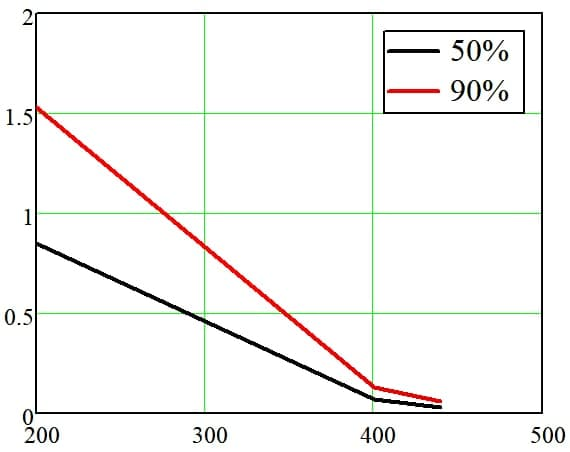
\includegraphics[width=0.4\linewidth]{2.jpg}}
		\label{ris2}
	\end{figure}
	\end{center}
	
	

%-----------------------------------------3
\begin{center}
\textbf{Завдання 3}
\end{center}




	На графіку <<Ciмейство кривих залежностi Енергiя(частота)>> по осi ігрек на мою думку -- це кiнетична енергiя, це можна зрозуміти якщо прочитати II закон Столетова.
















\end{document}